\chapter{Considerações Finais}

Considerando-se tudo o que foi apresentado até agora, a proposta de pesquisa e desenvolvimento para a continuação deste trabalho é a de utilização de dois métodos de Aprendizagem Incremental tendo como ponto de partida o problema do MAPA apresentado do capítulo anterior. Um modelo de Aprendizagem Incremental puro será escolhido e implementado para resolver o problema do sistema classificador. Paralelamente uma abordagem baseada no modelo lote-incremental será usada com um método clássico de AM. O objetivo final da próxima etapa deste trabalho é realizar um estudo comparativo entre estas duas abordagens, visando descobrir qual dos modelos apresentará melhor performance e adequação a resolução do problema. Além da acurácia das predições do modelo também serão avaliados os seguintes aspectos: Aplicabilidade em ambientes reais, complexidade de compreensão do modelo e facilidade de manutenção do sistema criado.

\section{Cronograma}
O cronograma da figura 14 é apresentado para o desenvolvimento das próximas etapas. 

\begin{figure}[!h]
\centering
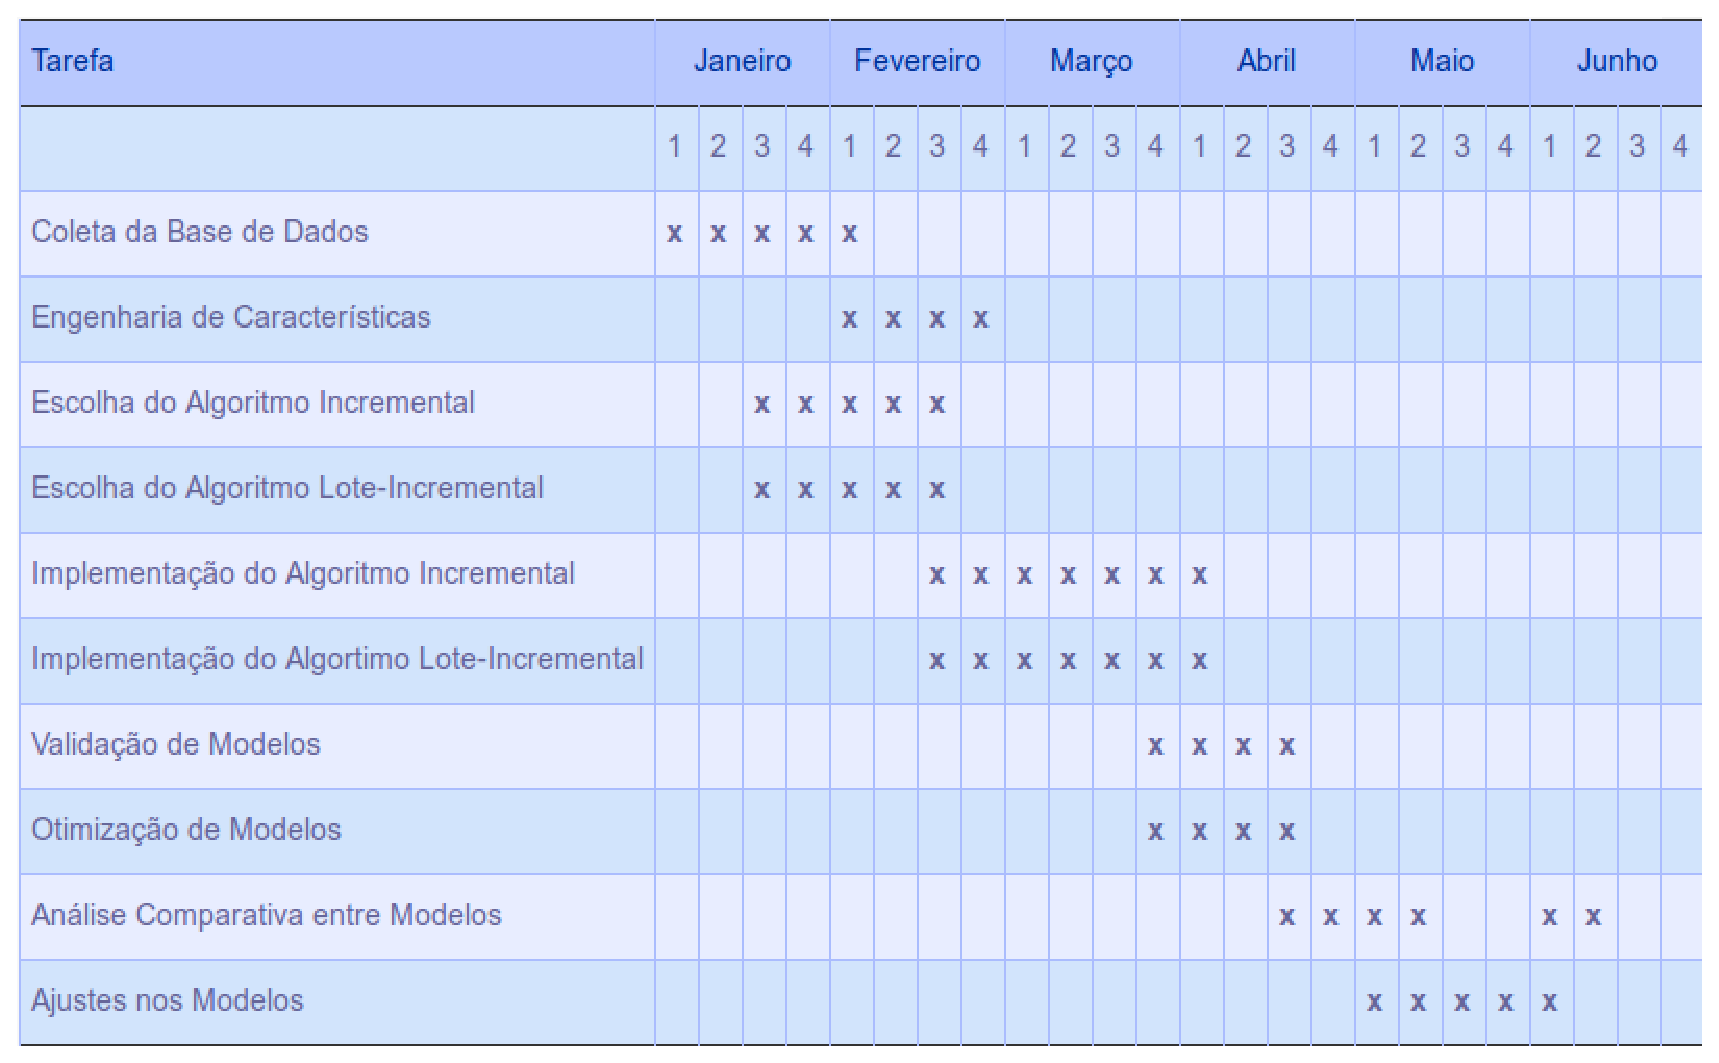
\includegraphics[keepaspectratio=true,scale=0.50]
{figuras/cronograma.eps}
\caption{Cronograma das Próximas Atividades}
\label{cronograma}
\end{figure}

Cada tarefa definida no cronograma consiste em:
\begin{enumerate}
\item Definição de Base de Dados: Concretização da utilização da base de dados do MAPA como caso problema para o desenvolvimento do trabalho. Avaliação da necessidade de inclusão de novas fontes de dados e problemas a serem atacados.
\item Coleta da Base de Dados: Coleta da(s) base(s) de dados definidas na tarefa anterior.
\item Engenharia de Características: Pré-processamento e análise dos conjuntos de dados que serviram como entrada dos modelos.
\item Escolha do Algoritmo Incremental: Pesquisa do estado da arte sobre algoritmos de AM com Aprendizagem Incremental e escolha de um deles que seja adequado a solução do problema.
\item Escolha do Algoritmo Lote-Incremental: Pesquisa do estado da arte sobre algoritmos que podem ser utilizados com uma abordagem lote-incremental e escolha de um deles para aplicação no trabalho.
\item Implementação do Algoritmo Incremental: Desenvolvimento do algoritmo incremental.
\item Implementação do Algoritmo Lote-Incremental: Desenvolvimento do algoritmo lote-incremental.
\item Validação dos Modelos: Análise de desempenho das predições realizadas pelos modelos.
\item Otimização dos Modelos: Aplicação de aprimoramentos nos modelos implementados.
\item Análise Comparativa entre Modelos: Análise comparativa entre os modelos adotados.
\item Ajustes nos Modelos: Ajustes finais nos modelos.
\end{enumerate}